\documentclass{beamer}
\usetheme{Madrid}
\usepackage[style=numeric, citestyle=numeric]{biblatex}
\addbibresource{references.bib}
\setbeamertemplate{bibliography item}[text]
\usefonttheme[onlymath]{serif}

%\usepackage{hyperref}   % Enable embedded hyperlinks.
\usepackage{graphicx}    % Enable for eps and pdf figures, if they occur
\usepackage{verbatim}   % Printing strings as is
\usepackage{mathtools}  % for correct NORM formatting
\usepackage{float}      % for H directive
\usepackage{xcolor}
%\usepackage{enumitem}   % for easily changing labels in enumerate env

\newcommand{\C}{\mathbb C} % blackboard bold , for ``complex,'' etc
\newcommand{\R}{\mathbb R} 
\newcommand{\Z}{\mathbb Z}
\newcommand{\Q}{\mathbb Q}
\newcommand{\N}{\mathcal N} % normal distribution
\newcommand{\D}{\mathcal D} % dataset
\newcommand{\E}{\mathbb E}
\newcommand{\G}{\mathcal G} % Graph
\newcommand{\V}{\mathcal V} % Vertices
\let\E\undefined
\newcommand{\E}{\mathcal E} % Vertices
\let\L\undefined
\newcommand{\L}{\mathcal L} % Label function


\DeclarePairedDelimiterX{\norm}[1]{\lVert}{\rVert}{#1} 
\DeclarePairedDelimiterX{\abs}[1]{\lvert}{\rvert}{#1}
\DeclarePairedDelimiterX{\ip}[2]{\langle}{\rangle}{#1, #2}
\DeclarePairedDelimiterX{\pfrac}[2]{(}{)}{\frac{#1}{#2}}
\DeclareMathOperator{\sign}{sign}
\DeclareMathOperator*{\argmin}{arg\,min\,} % the * places underscore arg below
\DeclareMathOperator*{\argmax}{arg\,max\,}
\DeclareMathOperator{\relu}{relu}
\DeclareMathOperator{\prox}{\mathbf{prox}} % proximal operator
\DeclareMathOperator{\dom}{\mathbf{dom}} % domain
\DeclareMathOperator{\bd}{\mathbf{bd}} % boundary of a set
\DeclareMathOperator{\epi}{\mathbf{epi}} % epigraph
\DeclareMathOperator{\tr}{\mathbf{tr}} % trace
\DeclareMathOperator{\rank}{\mathbf{rank}} % rank
\DeclareMathOperator{\diag}{\mathbf{diag}} % diagonal
\DeclareMathOperator{\conv}{\mathbf{conv}} % convex hull
\DeclareMathOperator{\Var}{\mathrm{Var}} % variance
\let\vec\undefined
\DeclareMathOperator{\vec}{\mathbf{vec}} % vectorization (flattening)
\let\pderiv\undefined
\newcommand{\pderiv}[2]{\frac{\partial #1}{\partial #2}}
\let\deriv\undefined
\newcommand{\deriv}[2]{\frac{d\, #1}{d\, #2}}

\title{Deep Graph Convolutional Networks}
\subtitle{Computer Vision Final Project}
\author{Nikola Janju\v{s}evi\'{c}}
\institute{NYU}
\date{December 17th 2020}

\AtBeginSection[]
{
	\begin{frame}
		\frametitle{Table of Contents}
		\tableofcontents[currentsection]
	\end{frame}
}

\begin{document}
\frame{\titlepage}

\newcommand{\mycite}[1]{\textit{\citetitle{#1}} \cite{#1}}
\begin{frame}{Today's Papers}
\begin{refsection}
	\nocite{*}
	\printbibliography[keyword=myprez]
\end{refsection}
\end{frame}

\section{Motivation}
\begin{frame}[allowframebreaks]{Motivation: graph representation of data}
\begin{itemize}
\item Irregular data domains: point clouds, sensor networks
	\begin{figure}[H]
	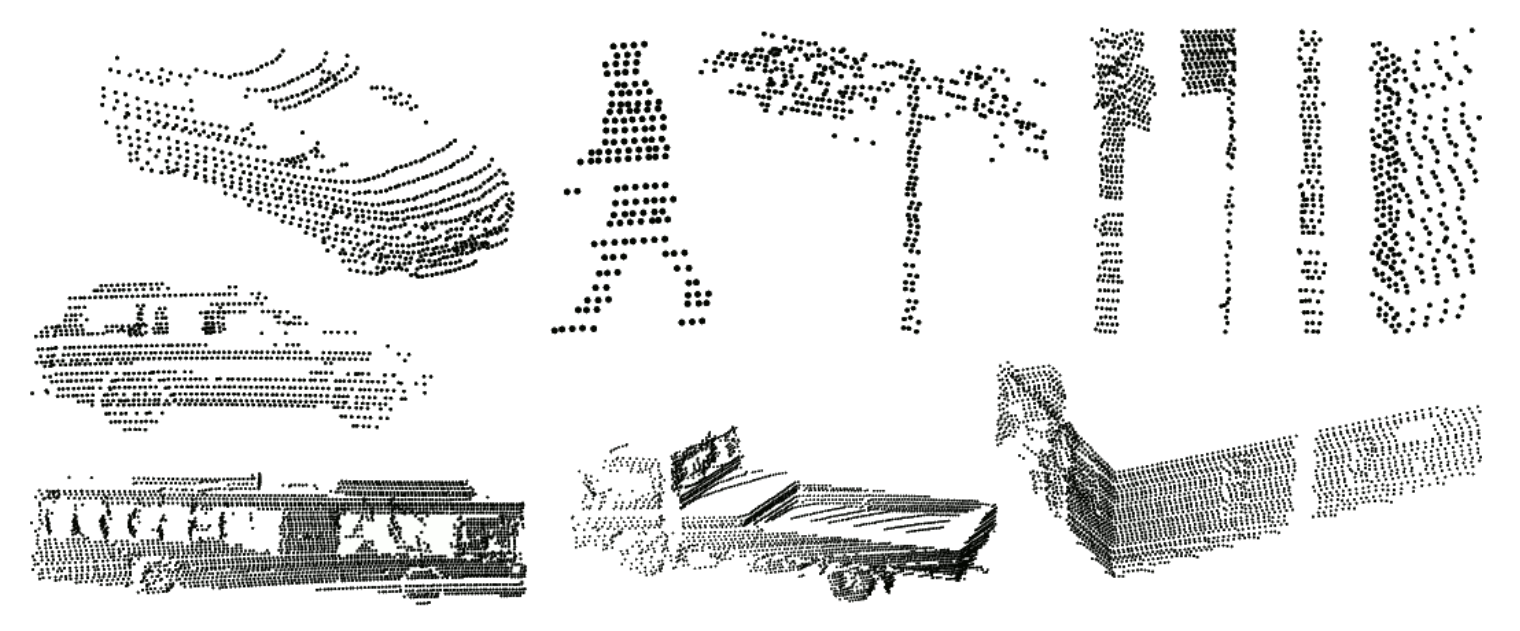
\includegraphics[width=0.8\textwidth]{../imgs/point_cloud.png}
	\caption{\cite{Simonovsky2017ecc}}
	\end{figure}

\newpage
\item Capture non-local relations in regular-domain data
	\begin{figure}[H]
	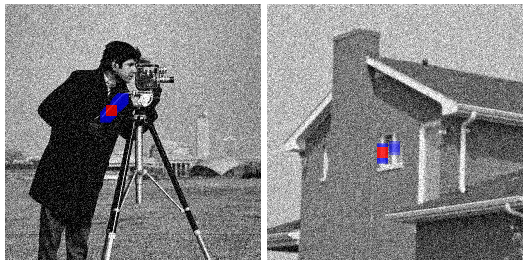
\includegraphics[width=0.8\textwidth]{../imgs/bm3d.png}
	\caption{\cite{BM3D}}
	\end{figure}
\end{itemize}
\end{frame}

\section{Convolution over Graphs}
\begin{frame}{Linear Convolution as a special case:}
\begin{figure}[H]
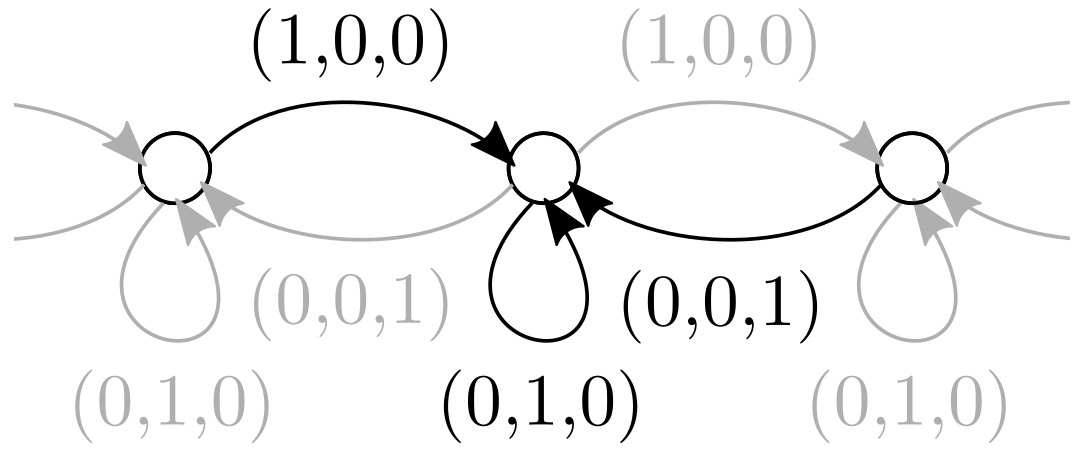
\includegraphics[width=0.8\textwidth]{../imgs/1DConv.png}
\caption{\cite{Simonovsky2017ecc}}
\end{figure}
\end{frame}

\begin{frame}{Frequency and spatial domain formulations}
\begin{itemize}
\item Notion of spectrum can be defined via Graph-Laplacian. Filtering then naturally arises.
\item Building/applying Graph-Laplacian can be expensive, not nice for dynamically changing graphs.
\item Spatial domain: define filtering as node/vertex signal agregation. Less expensive but no 
clear formulation.
\end{itemize}
\end{frame}

\begin{frame}{Notation}
Consider $x \in \R^{CN}$, a multi-channel signal with $N$ pixels.
\begin{itemize}
\item $x[i] \in \R^C$, feature vector of pixel $i$.
\item $x^k \in \R^N$, channel $k$ of $x$.
\item $\G(\V,\E)$ directed graph with vertices $\V$, edges $\E$.
\item $\V$ set of verticies, $\abs{\V}=N$
\item $\E$ set of edges $\E \subseteq \V \times \V$.
\item $\N(i) = \{j | (i,j) \in \E \}$ set of neighbors of vertex $i$. 
\item $\L: \E \rightarrow \R^{D}$ label map.
\item $\L[i,j] \in \R^D$ label for edge connecting vertex $j$ to $i$.
\end{itemize}
\end{frame}

\begin{frame}[allowframebreaks]{Edge Conditioned Convolution}
\begin{definition}[ECC \cite{Simonovsky2017ecc}]
Consider multi-channel  signal $x \in \R^{C_{in}N}$, 
and \textit{Label-Operator Mapping} $\mathcal{F}: \R^{M} \rightarrow \R^{C_{out}\times C_{in}}$. 
Define the \textit{Edge-Conditioned Convolution} of $x$ by $\mathcal{F}$ as
\begin{align}
y[i] &= \sum_{j \in \N(i)} \mathcal{F}(\L[i,j])x[j] \\
&= \sum_{j \in \N(i)} \mathbf{H}_{ij}x[j] \in \R^{C_{out}}
\end{align}
where we say $\mathbf{H}_{ij}$ is the \textit{edge-conditioned feature operator} from $j$ to $i$.
\end{definition}

\begin{itemize}
\item Consistent with multi-channel grid-convolution if $\mathbf{H}_{ij}$ is stationary 
(only function of $\tau = j-i$), though non-intuitive.
\end{itemize}

\newpage

\begin{itemize}
\item For 1D grid-convolution, $\mathcal{F}(\L[i,j]) = \ip{h}{e_{j-i}}$ ($e_k$ dim $k$ unit-vector), 
i.e. selecting coefficient $j-i$ from filter $h$.
\item When ordering of neighbors no-longer makes sense, stationary kernel can be abandoned. 
\item \cite{Simonovsky2017ecc} learn label-operator mapping $\mathcal{F}$ as 2-layer MLP
\item Other spatial graph-convolution formulations don't have grid-convolution as special case, 
don't handle multi-channel signals properly, and/or use uninformative edge-labels
\item \cite{Simonovsky2017ecc} set SOA results on point-cloud classification
\end{itemize}
\end{frame}

\section{Graph Convolutional Denoising Network (GCDN)}
\begin{frame}{GCDN}
\begin{itemize}
\item Dynamically build K-Nearest Neighbors graph in feature-space 
to exploit non-local similarities for denoising images (like BM3D)
\item Average local convolutions with non-local agregations over graph (ECC)
\end{itemize}
\end{frame}

\begin{frame}{Motivating Results \cite{ValsesiaICIP19}}
\begin{figure}[H]
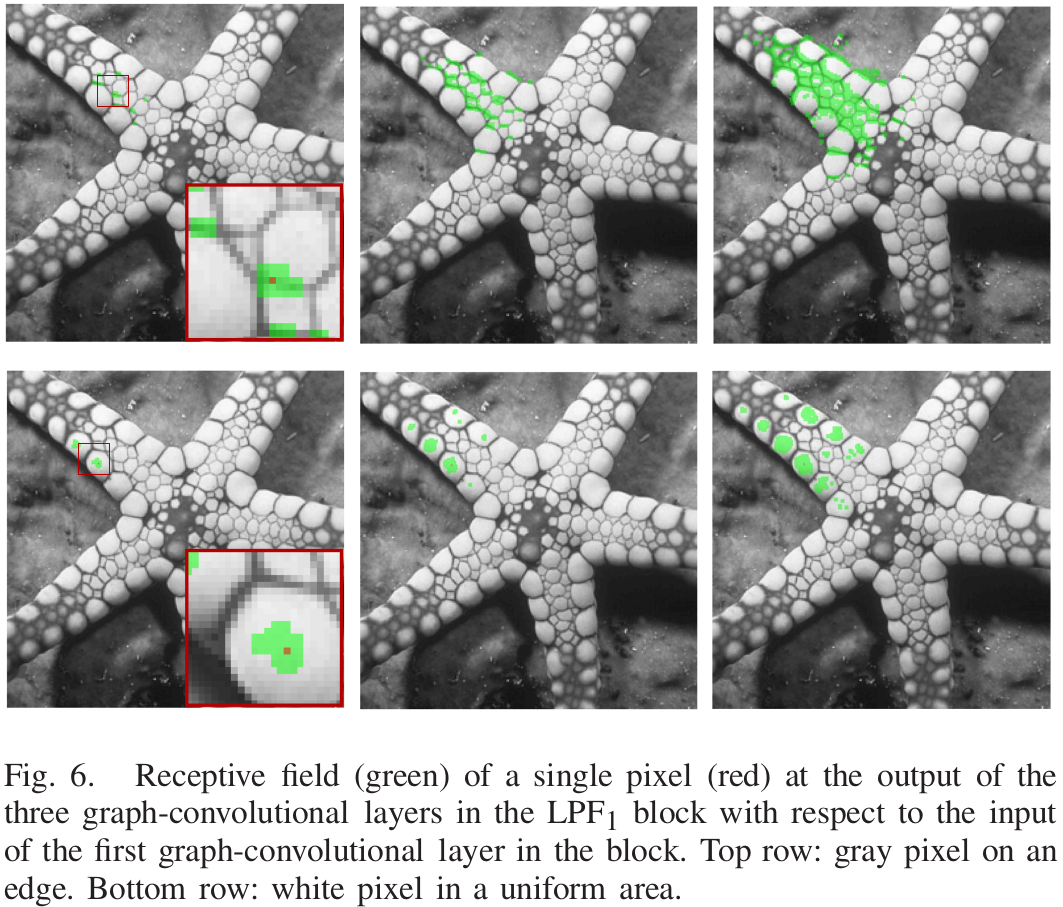
\includegraphics[width=0.75\textwidth]{../imgs/starfish_cap.png}
\end{figure}
\end{frame}

\begin{frame}{Architecture \cite{ValsesiaICIP19}}
\begin{figure}[H]
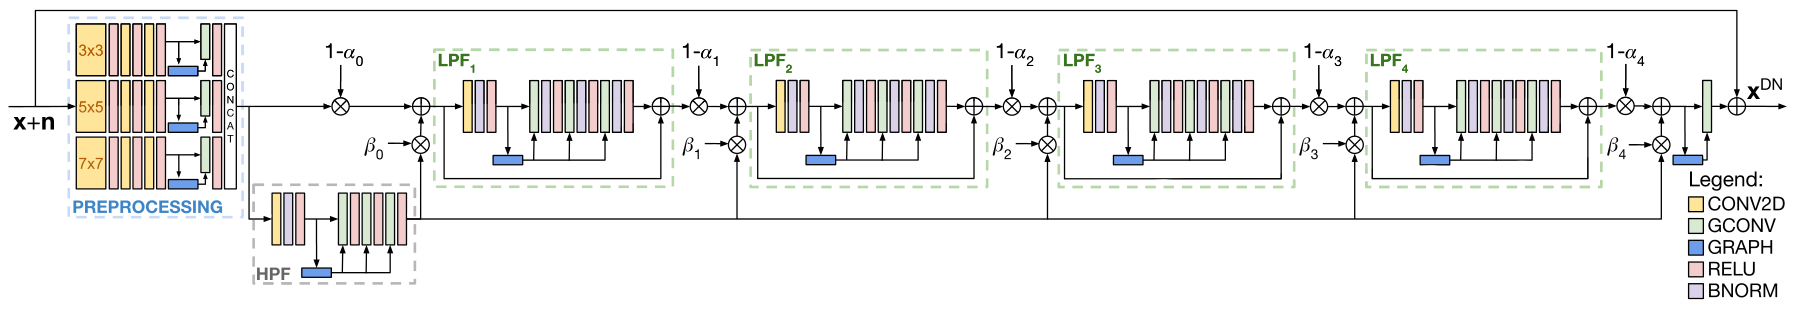
\includegraphics[width=1\linewidth]{../imgs/gcdn_arch.png}
\end{figure}
\begin{itemize}
\item Residual learning with batch-norm
\item Build KNN graph for each ``block'' (not every convolution)
\item All intermediate signals stay at same spatial resolution (no subsampling)
\item Can be (loosely) viewed as unrolled proximal gradient descent with graph-laplacian operator,
$$ \hat{x} = \argmin_{x} \frac{1}{2}\norm{\mathbf{A}x-y}_2^2 + \frac{\beta}{2}x^\top \mathbf{L}x $$
(for denoising $\mathbf{A} = \mathbf{I}$)
\end{itemize}
\end{frame}

\begin{frame}[allowframebreaks]{GConv Module \cite{ValsesiaICIP19}}
\begin{figure}[H]
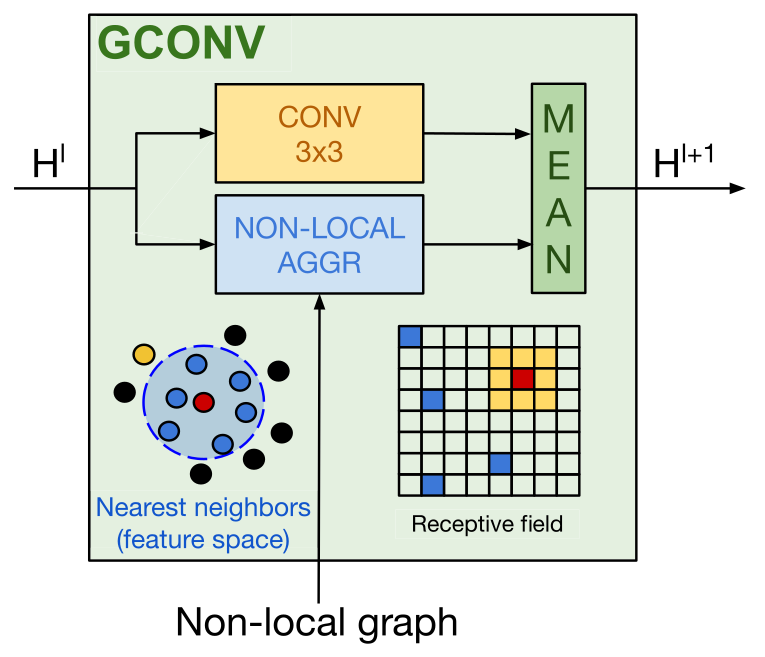
\includegraphics[width=0.3\linewidth]{../imgs/nlagg.png}
\end{figure}
\begin{itemize}
\item $$x^{(\ell+1)} = \frac{1}{2}\left( x^{(\ell+1),L} + x^{(\ell+1),NL} \right) + b^{\ell+1}$$
\item $x^{(\ell+1),L}$ local 3x3 convolution
\item $x^{(\ell+1),NL}$ non-local ECC,
\begin{align}
x^{(\ell+1),NL}[i] &= \sum_{j \in \N^{(\ell)}(i)} \mathcal{F}^{(\ell)}(\L^{(\ell)}[i,j])x^{(\ell)}[j] \\
&= \sum_{j \in \N^{(\ell)}(i)} \mathbf{H}^{(\ell)}_{ij}x^{(\ell)}[j]
\end{align}
\item Implement label operator map $\mathcal{F}$ as low-rank MLP, via sum of $r$ outer-products
\begin{figure}[H]
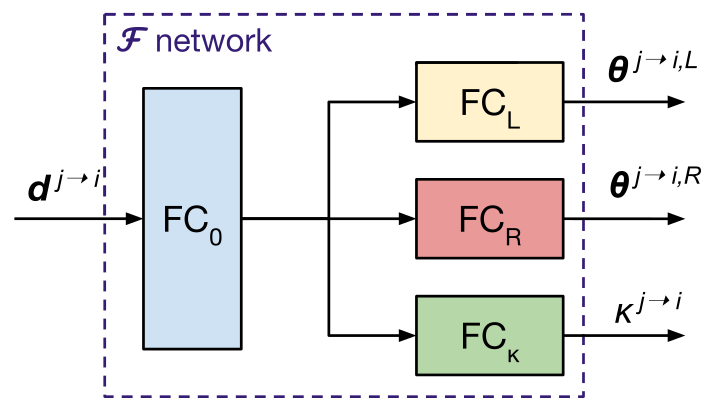
\includegraphics[width=0.3\linewidth]{../imgs/label_operator_map.png}
\end{figure}
\end{itemize}
\end{frame}

\begin{frame}{SOA Synthetic Denoising Results \cite{ValsesiaICIP19}}
\begin{figure}[H]
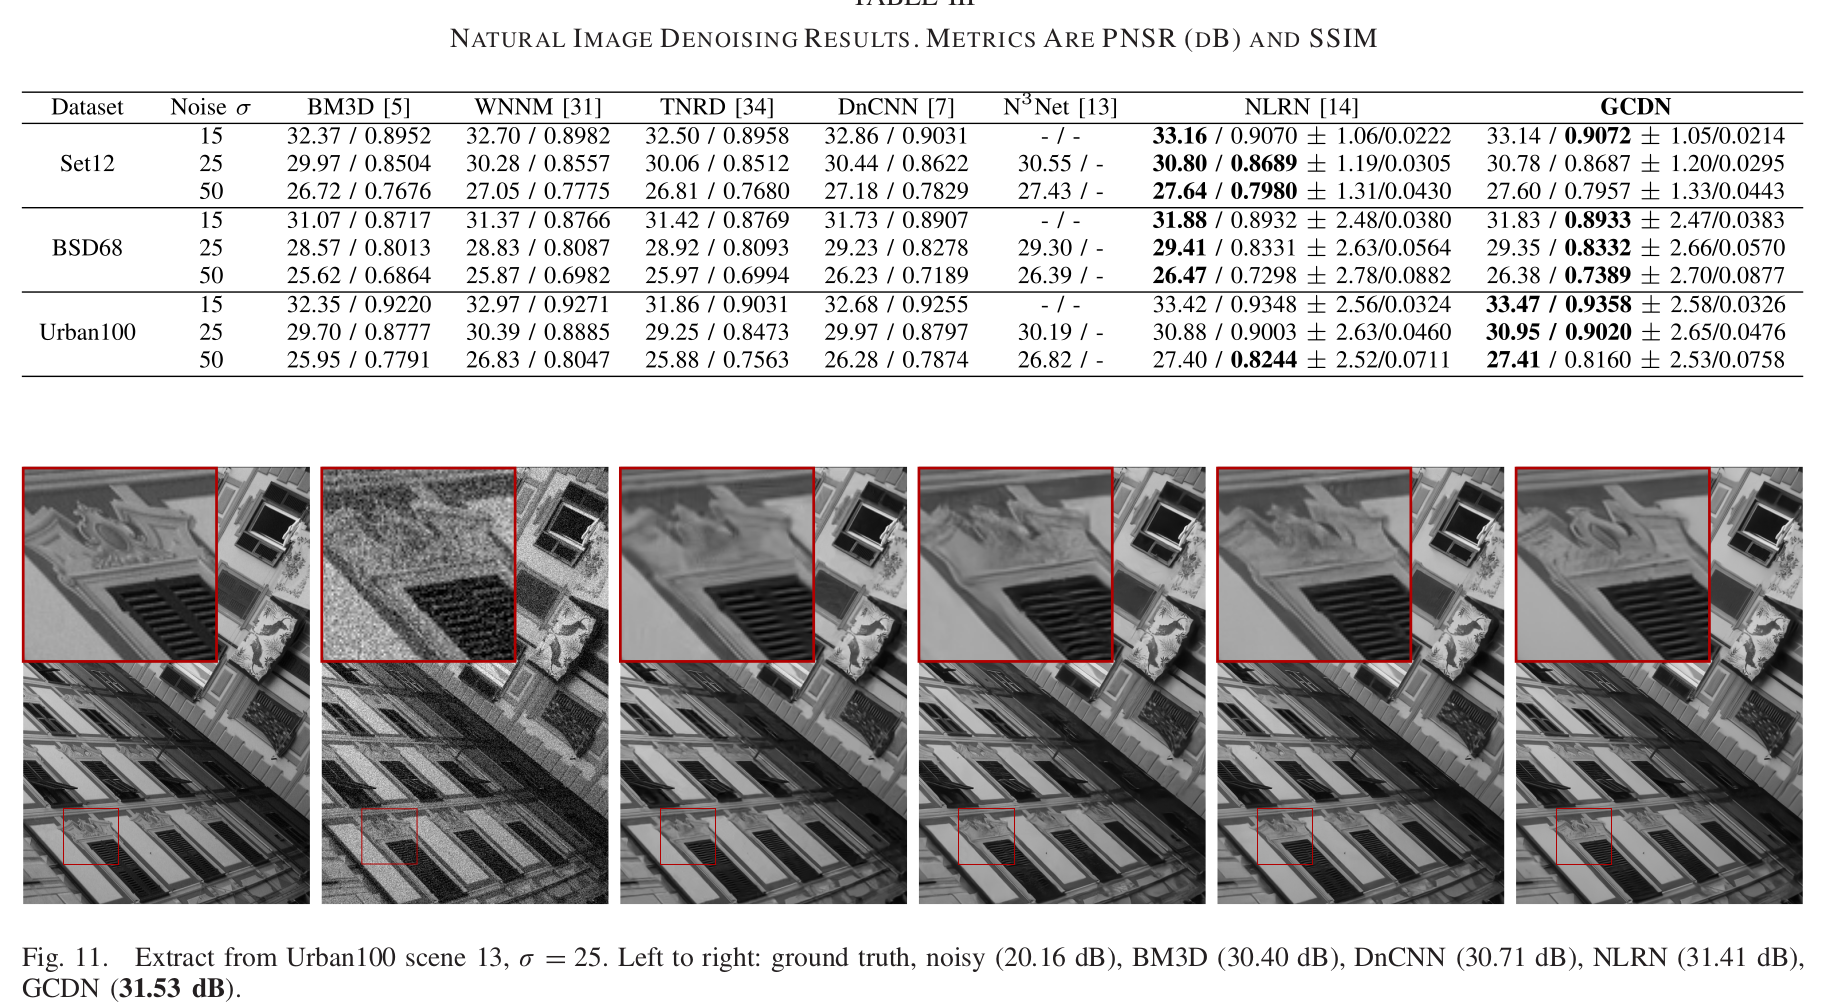
\includegraphics[width=\linewidth]{../imgs/soa_synth_000.png}
\end{figure}
\end{frame}

\begin{frame}{SOA Real Image Denoising Results \cite{ValsesiaICIP19}}
\begin{figure}[H]
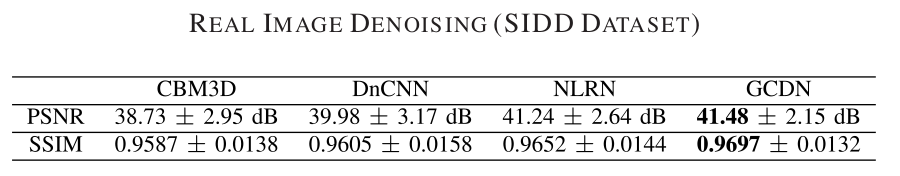
\includegraphics[width=0.8\linewidth]{../imgs/soa_real_table.png}
\end{figure}
\begin{figure}[H]
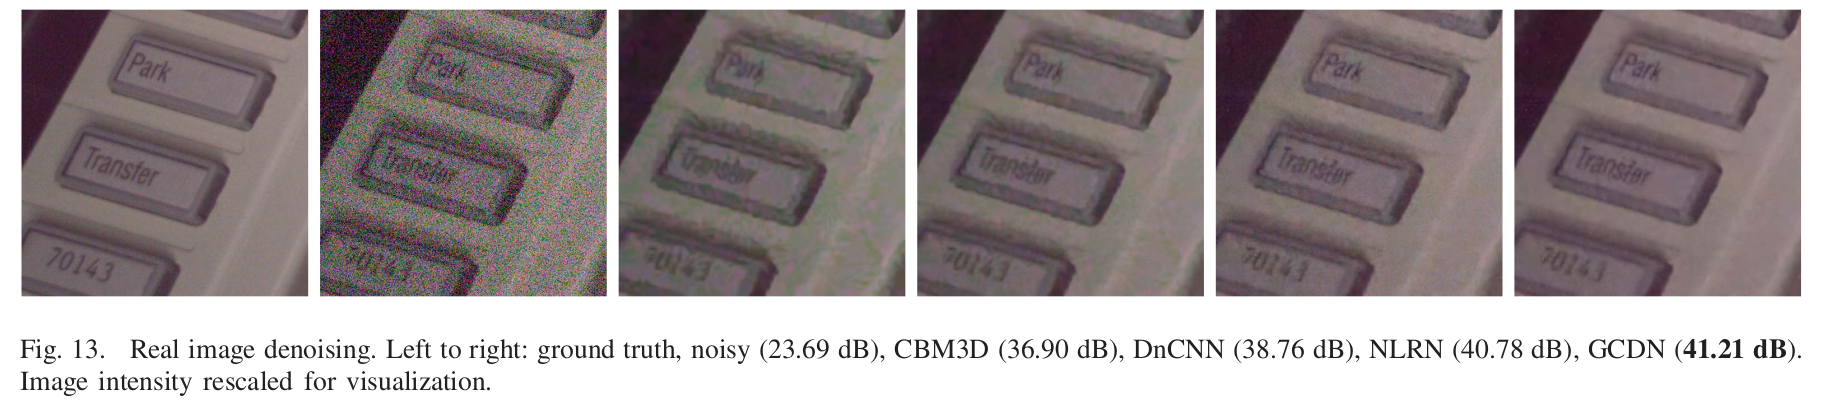
\includegraphics[width=\linewidth]{../imgs/soa_real.png}
\end{figure}
\end{frame}

\begin{frame}{Receptive Field: Learned feature-domain vs. image-domain}
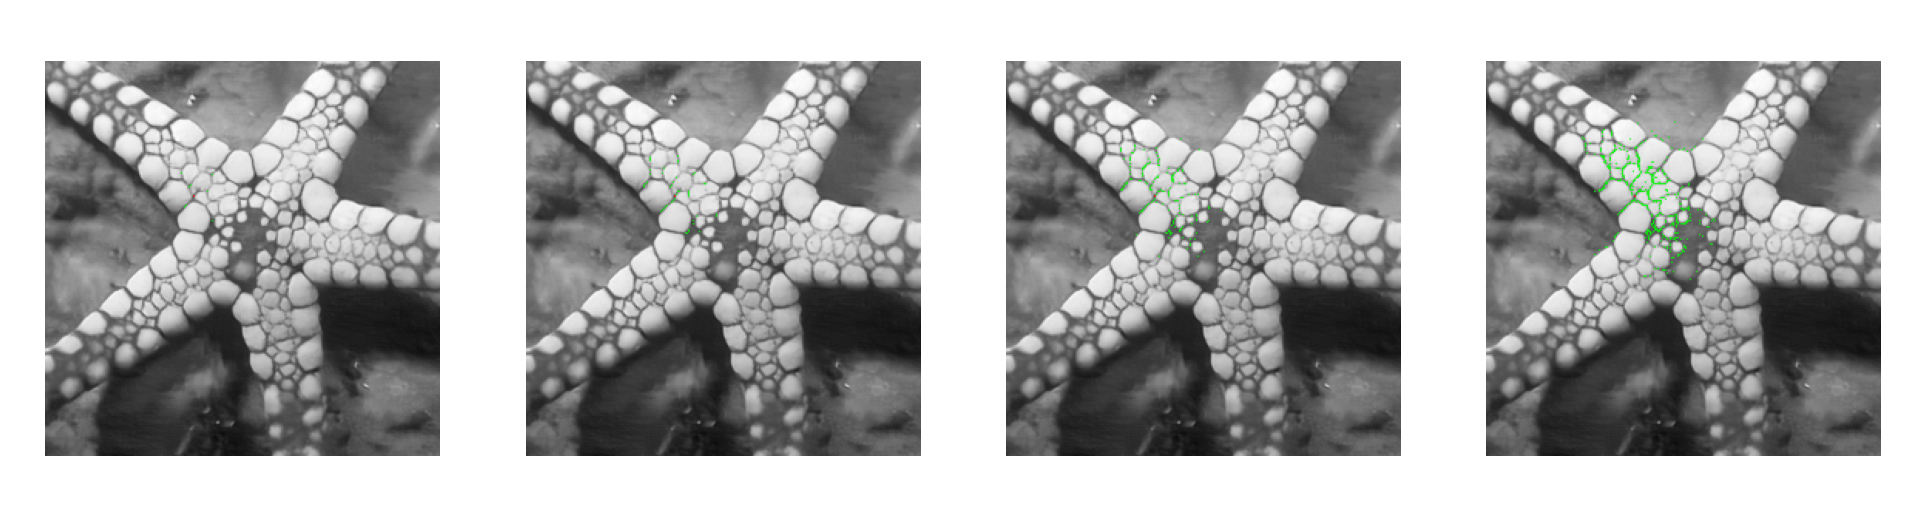
\includegraphics[width=\linewidth]{../imgs/my_receptivefield.png}
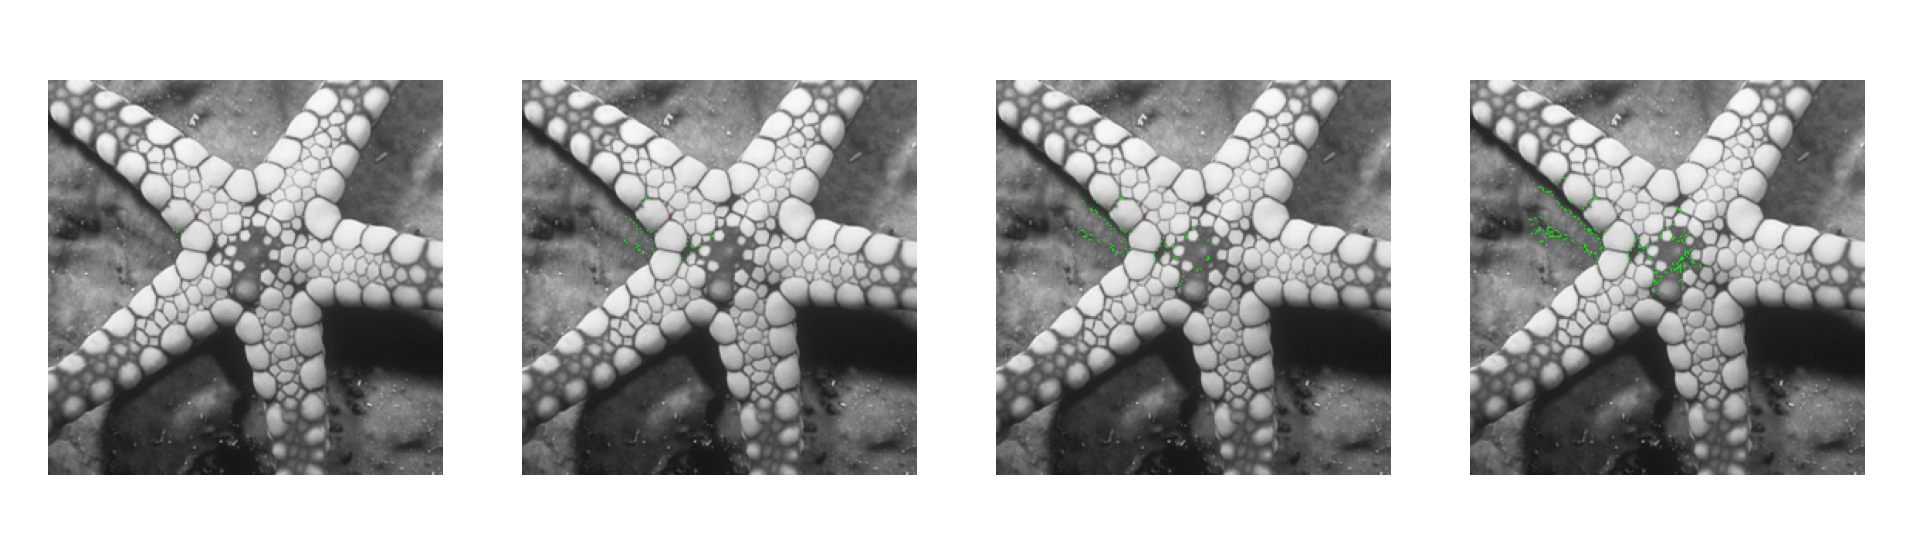
\includegraphics[width=\linewidth]{../imgs/dumb_receptivefield.png}
\end{frame}

\begin{frame}{Extensions}
\begin{itemize}
\item SOA Point-Cloud denoising \cite{PistilliECCV20}
\begin{figure}[H]
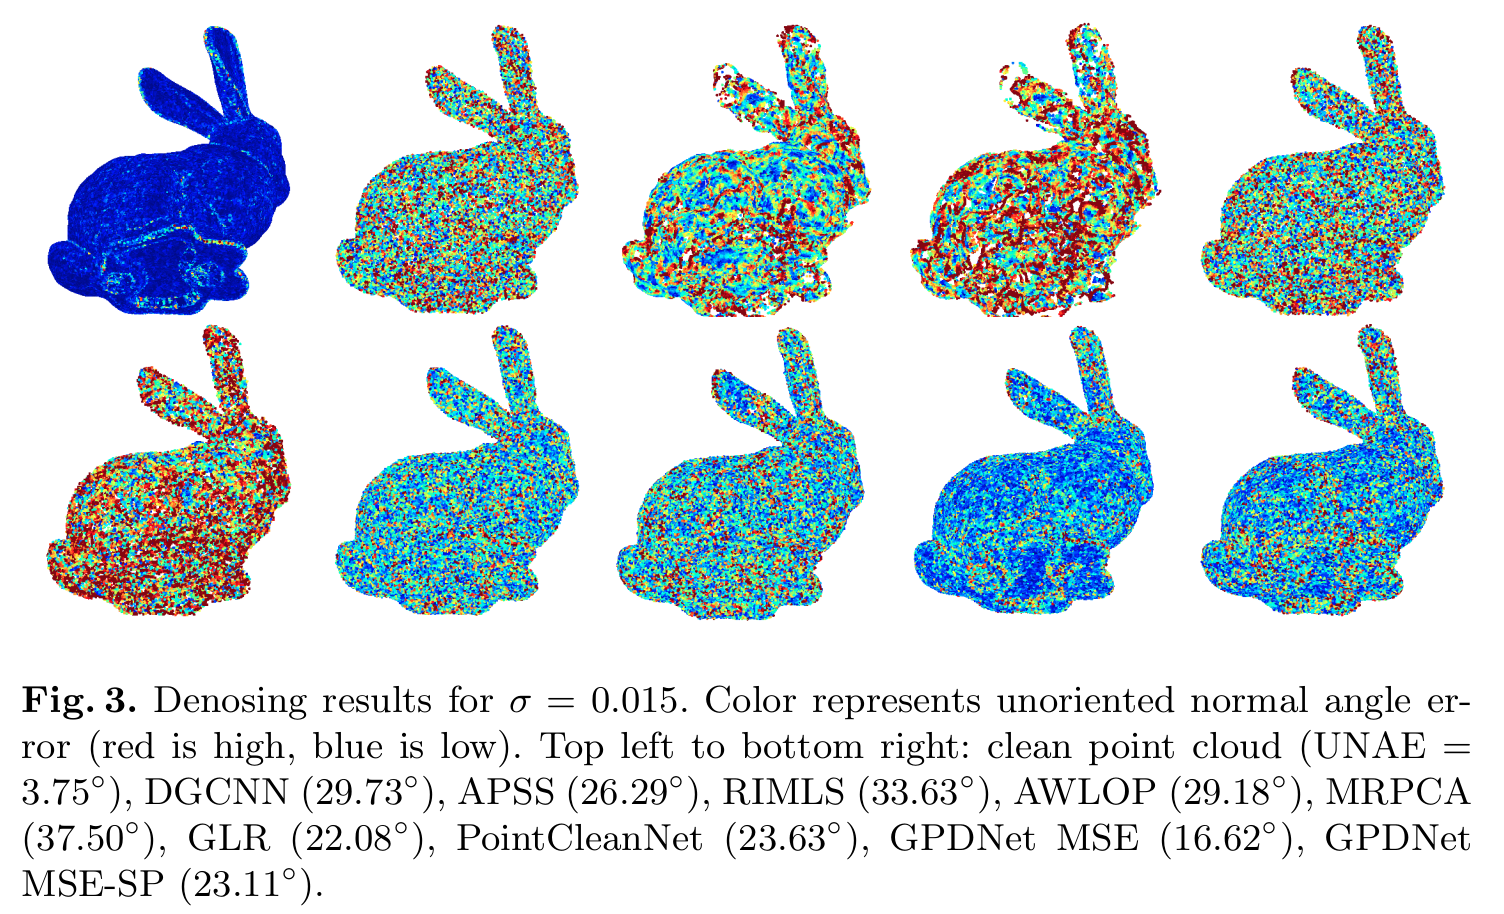
\includegraphics[width=0.5\linewidth]{../imgs/pcdn.png}
\end{figure}
\begin{figure}[H]
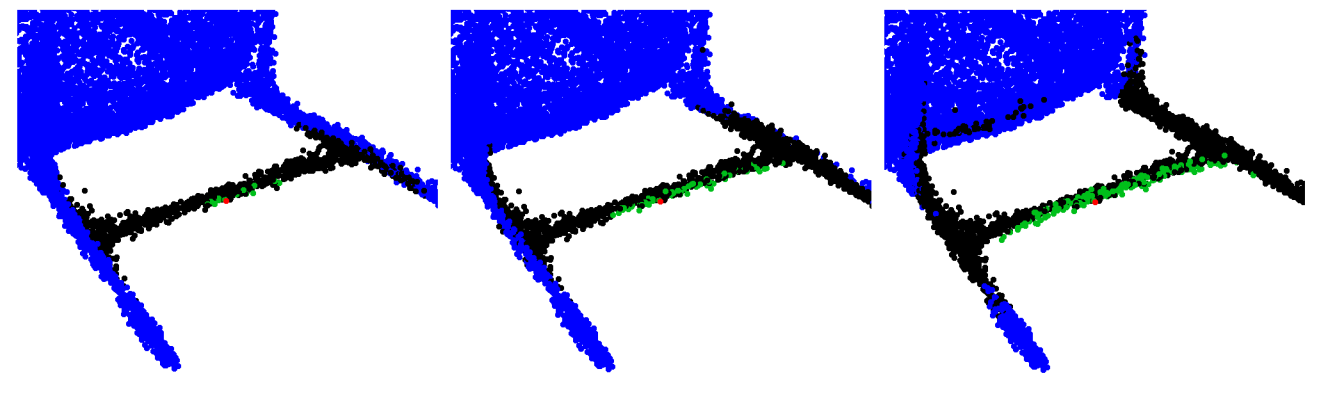
\includegraphics[width=0.5\linewidth]{../imgs/pcdn_receptive.png}
\end{figure}
\end{itemize}
\end{frame}

% Bibliography
\begin{frame}[allowframebreaks]{References}
\nocite{*}
\printbibliography
\end{frame}

\end{document}
